\section{Homework 2}

\subsection{问题1}

(a) 设最左上角的格子坐标为$(0,0)$, 最右下角为$(3,3)$, $X_{i,j}$为坐标$(i,j)$格子的
取值. 则$X=\{X_{0,1}, X_{0,2}, X_{1,1}, X_{1,2}, X_{2,1}, X_{2,2}, X_{3,0}, X_{3,3}\}$为状态集.
其中对于空的格子, $X_{i,j}\in D_{i,j}=\{1,2,3,4\}$, 对于已填好的格子$X_{i,j}$就取对应的数值.
则约束条件为$C=\{
    ((x_{i,0}, x_{i,1}, x_{i,2}, x_{i,3}), \text{alldiff}), \\
    ((x_{0,j}, x_{1,j}, x_{2,j}, x_{3,j}), \text{alldiff}),
    ((x_1,x_2,x_3,x_4)\text{在同一}2\times2\text{子网格内}), \text{alldiff}\}$

(b) 该问题的解如表\ref{tab:2-1}.

\begin{table}[htbp]
    \centering
    \begin{tabular}{*4{|c}|}
        \hline 
        1 & 2 & 4 & 3 \\\hline 
        4 & 3 & 1 & 2 \\\hline 
        2 & 4 & 3 & 1 \\\hline 
        3 & 1 & 2 & 4 \\\hline
    \end{tabular}
    \caption{2-1答案}\label{tab:2-1}
\end{table}

\subsection{问题3}

\begin{figure*}[htbp]
    \centering
    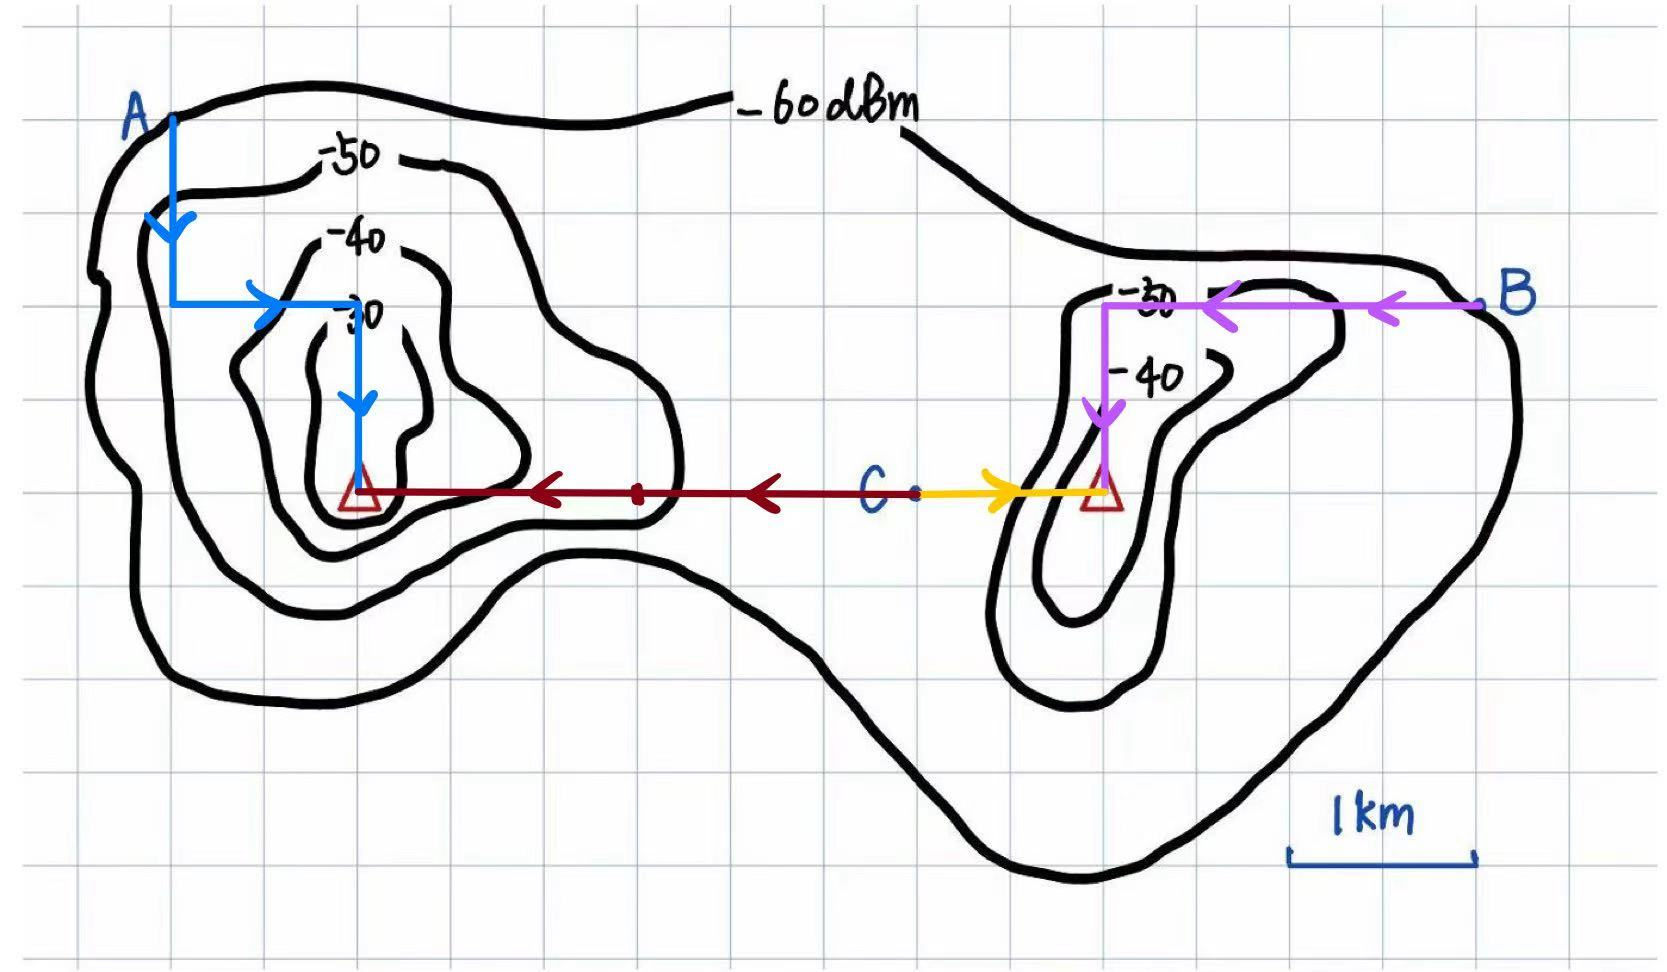
\includegraphics[width=0.7\textwidth]{images/2-3.jpg}
    \caption{2-3路径}\label{fig:2-2}
\end{figure*}

显然信号最强的区域为左侧信号塔.

(a) 无人机的寻路路径如图\ref{fig:2-2}蓝色路径所示, 可以到达.

(b) 无人机的寻路路径如图\ref{fig:2-2}紫色路径所示, 无法到达.

(c) 对于$m=1000$的情况, 如图\ref{fig:2-2}黄色路径所示, 无法到达; 对于$m=1500$的情况,
如图图\ref{fig:2-2}红色路径所示, 可以到达.

(d) (1) 选择合适的初始点. (2) 略微扩大局部搜索的范围, 防止落入局部最优解.